\documentclass[12pt]{article}


\usepackage{amssymb,amsmath,amsthm} 

%geometry (sets margin) and other useful packages
\usepackage[margin=1.25in]{geometry}
\usepackage{graphicx,ctable,booktabs}
\usepackage{booktabs}
\usepackage{cancel}

% Define my smaller twiddle
\newcommand{\apwsim}{\raisebox{0.2ex}{\scriptsize$\sim$\normalsize}} 

%Redefining subsections as problems
\makeatletter
\newenvironment{problem}{\@startsection
       {subsection}
       {1}
       {-.2em}
       {-3.5ex plus -1ex minus -.2ex}
       {2.3ex plus .2ex}
       {\pagebreak[3]%forces pagebreak when space is small; use \eject for better results
       \normalsize\bf\noindent{Problem }
       }
       }
       {%\vspace{1ex}\begin{center} \rule{0.3\linewidth}{.3pt}\end{center}}
       %\begin{center}\large\bf \ldots\ldots\ldots\end{center}
       }
\makeatother

% Change font size of sections
\makeatletter
\renewcommand\section{\@startsection{section}{1}{\z@}%
                                  {-3.5ex \@plus -1ex \@minus -.2ex}%
                                  {2.3ex \@plus.2ex}%
                                  {\normalfont\large\bfseries}}
\makeatother

%Fancy-header package to modify header/page numbering 
\usepackage{fancyhdr}
\pagestyle{fancy}
\lhead{Price-Whelan}
\chead{} 
\rhead{\thepage} 
\lfoot{\small\scshape Astronomy Lab 1} 
\cfoot{} 
\rfoot{\footnotesize } 
\renewcommand{\headrulewidth}{.3pt} 
\renewcommand{\footrulewidth}{.3pt}
\setlength\voffset{-0.25in}
\setlength\textheight{648pt}

%%%%%%%%%%%%%%%%%%%%%%%%%%%%%%%%%%%%%%%%%%%%%%%

\begin{document}

\title{Height of Pupin}
\author{Adrian Price-Whelan}
\date{}%\small Revision: \today}

\maketitle

\thispagestyle{empty}

%Example problems
\section{Introduction}

\indent\indent Today we will spend the first part of the lab discussing and coming to understand the difference between \emph{errors} and \emph{uncertainties} in measurements. Progress in science is an iterative process that relies on making observations (taking data) and describing the world we see with mathematics (developing theories) -- but not necessarily in that order! Learning how to properly record measurements and how to represent your degree of uncertainty in those measurements is a fundamental skill for the sciences.  

\begin{problem}{ }
	\textit{Discuss the following questions with your lab partner and write your conclusions and thoughts in your lab notebook.}  \\ \\
	\textbf{You measure the length of your hand with a ruler that only shows inches: } \\
	\indent\textbf{How do you represent your measurement?} \\
	\indent\textbf{How well do you trust that number? (e.g. within 0.5~in? 1~in?)} 
\end{problem}

\subsection{Accuracy vs. Precision}
\begin{description}
	\item[Accuracy]: How close a measurement is to the ``true'' value.
	\item[Precision]: How close a measurement is to other measurements of the same quantity. 
\end{description}

\begin{center}
	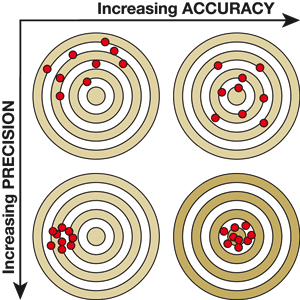
\includegraphics[scale=0.5]{precision_accuracy.png}
\end{center}

\subsection{Error vs. Uncertainty}

\indent\indent In most cases, measurements of some physical process cannot have infinite precision -- that is, you will always have some uncertainty in a number you measure. That uncertainty can either come from imperfect equipment or from random processes that conspire to cause some scatter in your results -- the difference is subtle, but let's take a moment to understand the difference. 
\begin{description}
	\item A \textbf{systematic error} is an error inherent to the experimental setup which causes some change in the results.
	\item A \textbf{random error} is an error inherent to the experimental setup which causes some change in the results.
\end{description}

Imagine your friend tells you to meet her at a bar at 10:00. You plan perfectly so you have time to get ready, and leave with enough time to get there. In fact, by your watch you arrive at precisely 10:00 -- but the bar is closed. What happened? You compare your watch to a stranger on the street and find that your watch is 6 hours behind! This is an example of a \emph{systematic} error -- you did everything right, but you relied on a piece of equipment (your watch) which skewed your arrival time.

Let's say you can't fix your watch, but it stays 6 hours behind -- you call your friend and explain what happened, and say that tomorrow you will account for this offset and be at the bar at 10:00PM. The next day, you figure out exactly what time you need to leave in order to make up for your screwy watch. Everything is going as planned, except the subway you get on gets delayed by 4 minutes. You arrive at the bar at 10:04PM -- not perfect because we can never truly predict whether the subway will be early or late, but at least this time you get to meet up with your friends. This is an example of a \emph{random error}.

\textbf{The bottom line:} a systematic error is anything that can be accounted for in your experiment and corrected for, whereas a random error can never be modeled because it comes from an inherently random process.

\subsection{Error Propagation}
\indent\indent What do you do if you make several measurements, and want to combine them via some equation to infer another quantity? For example, let's say you want to measure the speed of a car on the highway. We draw two lines on the highway and measure the distance between the two lines to find that they are \apwsim32~m apart -- but our meter stick didn't have millimeters, so I estimate that the value and uncertainty is actually:
\begin{equation}
	\Delta D = 32.5\pm0.2~m
\end{equation}
The next piece of information we need is the time it takes for the car to get from one line to the other. To get this, we use a stopwatch. We start and stop the stopwatch when the car is over the first and second lines, respectively, and see that the stopwatch reads 1.21 seconds -- but to account for our reaction speed, let's say we measure:
\begin{equation}
	\Delta t = 1.2\pm0.1~s
\end{equation}

Now we can calculate the velocity ($v = \Delta D/\Delta t$) -- but what do we do about the fact that both of our measurements have some associated uncertainty? To answer that, we have to understand how uncertainties \emph{propagate}.

\begin{description}
\item[Multiplying by a Constant:] If a result $Y = C \times X$, where $X$ is our measurement and $C$ is a known constant (e.g. 2 or $\pi$), then the uncertainty propagates as (where $\delta X$ is the uncertainty in X):

\begin{equation}
\delta Y = c \times \delta X
\end{equation}

For instance, is you measure the diameter of a pizza with an uncertainty of one millimeter, you know the circumference ($C = \pi \times d$) to an uncertainty of $\pi$ millimeters.

\item[Adding or Subtracting:] If you add (or subtract) two measurements to get a result, $Z = X + Y$, where $X$ and $Y$ are two measured quantities, the resultant error is found with
\begin{equation}
\delta Z = \sqrt{ \delta X^2 + \delta Y^2 }. 
\end{equation}

For example, if you know the mass of a bike to a precision of 4 pounds, and you know the mass of the rider to a precision of 3 pounds, you know the mass of the combined bike and rider to a precision of $\sqrt{4^2 + 3^2 } = 5$ pounds.

\item[Multiplying or Dividing:] If you multiply (or divide) two measurements $Z = X \times X$, where $X$ and $Y$ are both measurements and $Z$ is your result, the errors propagate according to
\begin{equation}
\frac{ \delta Z }{Z}= \sqrt{ \left( \frac{\delta X}{X} \right)^2 + \left( \frac{\delta Y}{Y} \right)^2 } .
\end{equation}
\end{description}

\begin{problem}{ }
	\begin{description}
		\item \textit{Discuss the following questions with your lab partner and record your work and results in your lab notebook.} 
		\item \textbf{You measure the height of the Empire State Building to be $1200 \pm 100$ feet, and the height of its antenna to be $300 \pm 40$ feet. What is the total height of the building and antenna, and the uncertainty in that result?}
		\item \textbf{From the above example about computing the velocity of the car, what would the velocity and uncertainty be given the measurements of $\Delta D$ and $\Delta t$?}
	\end{description}
\end{problem}

\section{Designing an Experiment}
Materials: tennis balls, meter sticks, rulers, twine, scissors, tape, mirrors, etc.

With your group, come up with three methods of measuring the height of Pupin with the materials you have been provided, and record the procedure for each in your notebook. How will you determine the precision of your measurements? \textbf{Show me your proposed methods to me before proceeding!}

\section{Measure the height of Pupin}
\indent\indent Once you have our approval, use only two of your measurement techniques to actually make measurements. For each technique determine a single value for the height of Pupin and the precision of that measurement.

When we've all finished, we'll come together as a group and compare our answers. Afterwards, in light of the group's conclusions, answer the following questions:

\begin{problem}{ }
	\begin{description}
		\item \textit{Answer in your notebook, utilizing the principals of good measurements we discussed today:} 
		\item \textbf{Which technique do you think worked best, and why?}
		\item \textbf{Determine a final value of the height of Pupin and the precision of that value.}
	\end{description}
\end{problem}

\end{document}